\chapter{Identification-Modélisation du système}
Dans un premier temps, nous allons déterminer les paramètres du moteur, ensuite, nous déterminerons le modèle fréquentiel ainsi que le modèle espace d'état du système. Puis, nous étudierons les propriétés, les performances et la stabilité du système. 
	\section{Détermination de paramètres et du retard}
	On identifiera les paramètres du moteur grâce à une approche dite \emph{boite noire}, c'est-à-dire que suivant la forme d'une réponse du système à un échelon, nous allons choisir une modélisation par fonction de transfert type (1\ier ordre, 2\ieme ordre, ...). Comme il s'agit d'un moteur à courant continu, nous choisissons un modèle du premier ordre car il permet de former un modèle de précision suffisante au vu de notre application.\\
Un modèle du 1\ier ordre est de la forme suivante :
\begin{equation}
G(p) = \frac{K}{\tau p+1}
\end{equation}
Où : 
\begin{description}
\item[$K$ :] Le gain statique du système.
\item[$\tau$ :] La constante de temps du système (en seconde).
\end{description}

\noindent Nous identifierons $K$ en mesurant le gain statique  de la réponse à un signal échelon (pour $t$ tel que la réponse se soit stabilisée): $ K = V_g(t)/U_m(t)$.\\
\noindent Pour l'estimation de $\tau$, nous utiliserons la relation suivante : $ \tau = t$ lorsque $\frac{V_g(t)}{U_m(t)} = 0,63*K $.\\

Pour identifier le retard, que nous savons être sur la commande du moteur, nous allons étudier de déphasage entre un signal d'entrée de type rectangle à fréquence faible ($1$Hz) et la sortie $V_s(t)$. Nous savons analytiquement qu'un système du premier ordre à un déphasage nul à basse fréquence, donc à partir du déphasage mesuré nous pouvons obtenir le retard.

	\section{Autres méthode}
Une autre façon de modéliser le modèle du moteur est un approche de type \emph{boite blanche}, c'est-à-dire de créer un modèle du moteur à partir d'une étude physique du système. 
	\section{Modèle fréquentiel}
Avec l'estimation des paramètres du moteur, nous avons former deux fonctions de transferts. La première définie le la fonction entre $V_g(t)$ et l'entrée $U_m(t)$ et la seconde entre $V_s(t)$ et $U_m(t)$. 
\begin{equation}
\left\lbrace
\begin{array}{l c l }
\frac{V_g(t)}{U_m(t)} 	&=& 	\frac{k_g \cdot k_m}{\tau_m p + 1	}e^{-hp}\\
&&\\
\frac{V_s(t)}{U_m(t)} 	&=& 	\frac{k_s \cdot k_m \cdot k_r}{ p\left(\tau_m p + 1\right)	}e^{-hp}\\
\end{array}
\right.
\end{equation}
Avec l'estimation des paramètres donnés en cours, figure \ref{fig:repIndiFTsEE} tracé (1) , nous avons tracer la réponse à un échelon unité de ces deux fonctions de transferts.
	\section{Modèle espace d'état}
À l'aide des fonctions de transferts précédentes, nous avons fait un modèle espace d'état en choisissant : \\
\begin{description}
\item[Pour entrée $u(t)$ :] $u(t) = U_m(t) $
\item[Pour sorties $y(t)$ :] $ y(t) = \begin{pmatrix}
V_g(t) \\
V_s(t)
\end{pmatrix}$
\item[Pour état $x(t)$ :] $x(t) = \begin{pmatrix}
\Theta_s(t)\\
\Omega_m(t)
\end{pmatrix}$
\end{description}
Nous avons extrait les équations suivantes du modèle schéma-bloc du moteur :
\begin{equation}
\label{eq:VsVgModel}
\left\lbrace
\begin{array}{lcl}
V_g(t) 	&=&		k_g \Omega_m(t)\\
V_s(t) 	&=&		k_s \Theta_s(t)\\
\end{array}
\right.
\end{equation}

Après manipulation des fonctions de transferts précédentes et des expressions de l'équation \ref{eq:VsVgModel}, nous avons obtenu le modèle espace d'état suivant : 
\begin{equation}
\label{eq:EE}
\begin{array}{lcl}

\left\lbrace
\begin{array}{l c l c lc}
\dot{x}(t) 
&=& 
A&
x(t) +& 
B &u(t-h)\\
&&&&\\

y(t) 
&=& 
C&
x(t) +& 
D &u(t-h)\\
\end{array}
\right. 

& \Rightarrow &

\left\lbrace
\begin{array}{l c l c lc}
\dot{x}(t) 
&=& 
\begin{bmatrix}
0	&	k_r\\
0	&	-\frac{1}{\tau_m}
\end{bmatrix}&
x(t) +& 
\begin{bmatrix}
0 \\
k_m
\end{bmatrix} &u(t-h)\\
&&&&\\

y(t) 
&=& 
\begin{bmatrix}
0	&	k_g\\
k_s	&	0
\end{bmatrix}&
x(t) +& 
\begin{bmatrix}
0 \\
0
\end{bmatrix} &u(t-h)\\
\end{array}

\right.
\end{array}
\end{equation}
À l'aide des paramètres de référence, nous avons tracé la réponse à un échelon unité du modèle espace d'état, figuere \ref{fig:repIndiFTsEE}, tracé (2).
\begin{figure}[!ht]
\centering
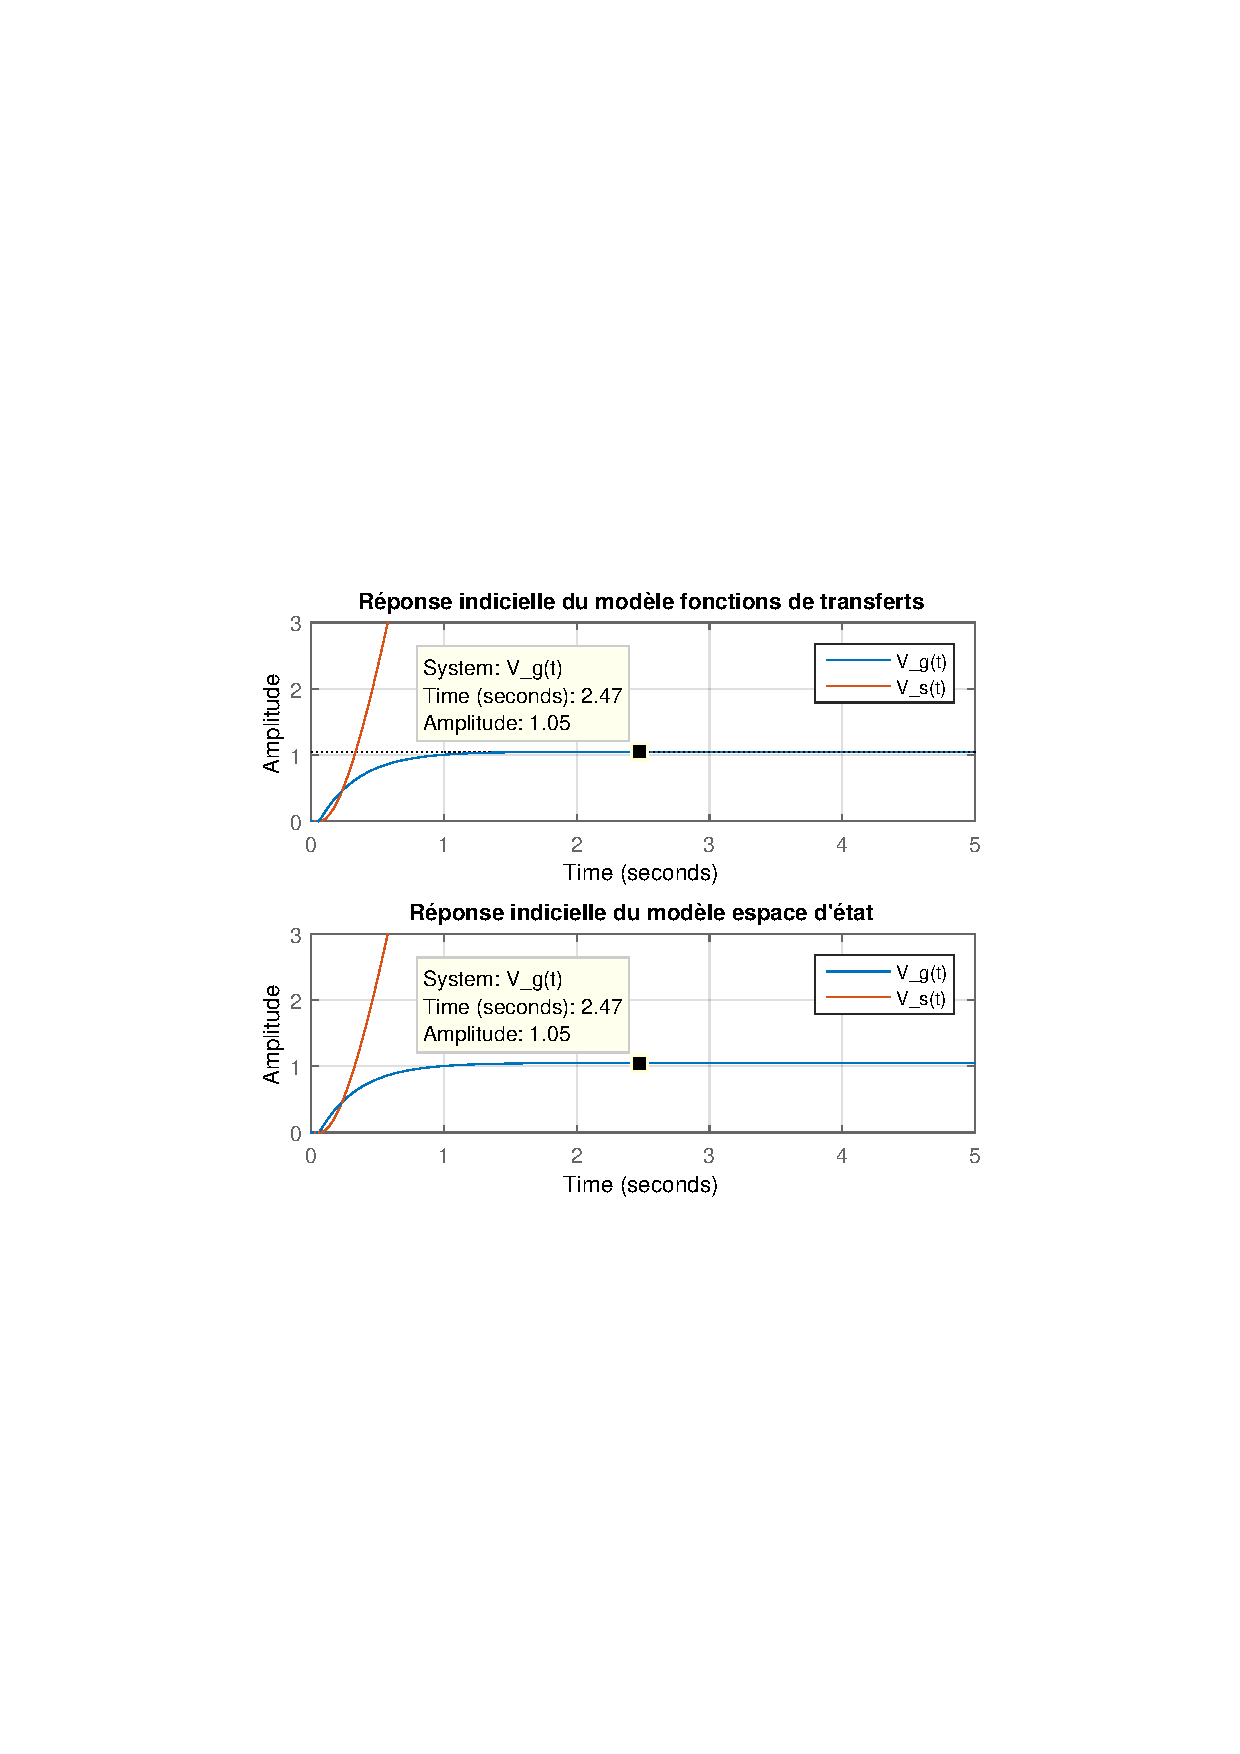
\includegraphics[width=.7\textwidth]{./I/images/modeles_ft-ee.pdf}
\caption{\label{fig:repIndiFTsEE}Réponse à un échelon indiciel des modèles fonctions de transfert (1) et espace d'état (2).}
\end{figure}

Nous avons comparé les réponses entres les deux modélisations afin de vérifier qu'il n'y ai pas d'erreur. Nous avons pour cela tracé la réponse à un échelon unité de la différence des deux modèles, figure \ref{fig:errFT_EE}
\begin{figure}[!ht]
\centering
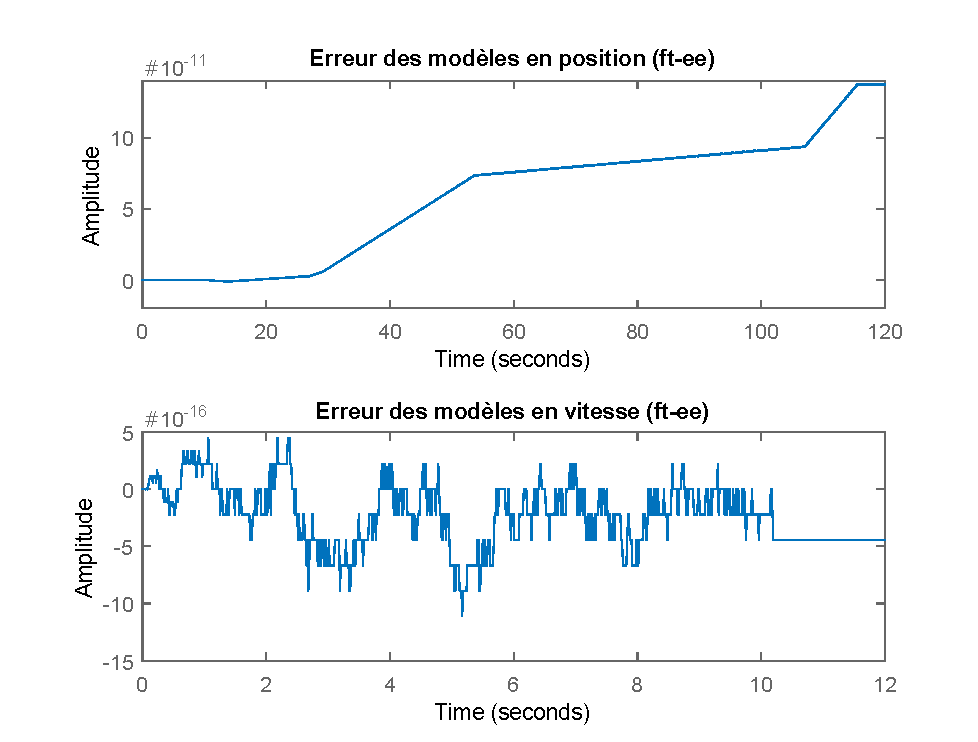
\includegraphics[width=.7\textwidth]{./I/images/erreurs_modeles_ft-ee.pdf}
\caption{\label{fig:errFT_EE} Réponse à un échelon unité de la différence des deux modèles.}
\end{figure}
Nous pouvons constater que l'erreur est négligeable et doit être dût à du bruit numérique et/ou à la méthode de calcul de la réponse. Nos modèles sont donc équivalents par rapport à une réponse à un échelon unité.
	\section{Commandabilité et observabilité}
Nous allons maintenant étudier l'observabilité et la commandabilité de notre modèle. Nous utiliserons, pour cela, le modèle espace d'état et matlab pour résoudre ce point. Nous avons vérifié que le rang de la matrice de commandabilité et de celle d'observabilité sont bien égaux à la dimension de $A$. Ces calculs nous permettent de conclure que le système est observable et commandable.
	\section{Analyse de la boucle ouverte}
Nous allons maintenant étudier les performances de notre système. Nous avons choisi d'étudier les performances sur la sortie $V_g(t)$. 
Toujours à l'aide de matlab, nous avons obtenu les performances suivantes : 
\begin{description}
\item[Temps de monté :] $t_m = 0,659 $ secondes.
\item[Temps de réponse à 5\% :] $t_r = 0,959$ secondes.
\item[Oscillation :] Il n'y a pas d'oscillations.
\item[Gain statique :] $G_{stat}= 1.05$. Il y a donc un dépassement de $0,05$ soit de $5\%$.	
\end{description}	
	\section{Stabilité de la boucle fermée}
	Est-ce bien ces deux méthodes ? (la troisième méthode supposée étant le pseudo-retard non traité en cours)
		\subsection{Delay-Sweeping}
		\subsection{Stabilité 2D}


